
%% dot -Tpng exampleLR0M.gz -o exampleLR0M.png
%%
%%  
%%

\documentclass[11pt,a4paper]{article}

\usepackage[american]{babel}
\usepackage[pdftex]{hyperref}
\usepackage{times}
\usepackage[T1]{fontenc}
\usepackage[margin=1in]{geometry}
\usepackage{amsmath}
\usepackage{graphicx}
\usepackage{tikz}
\usetikzlibrary{arrows,automata}
\usetikzlibrary{shapes.multipart}
\usetikzlibrary{shapes.misc}

\begin{document}

\renewcommand{\contentsname}%
	{Table of Contents}
\renewcommand{\abstractname}%
	{abstract}
\sloppy
\title{PTG(beta) User Manual}
\author{Egill B�i Einarsson}
\maketitle

\begin{abstract}
PTG is a command-line program that generates files containing parsing tables and state machines for a given grammar. Generated tables are in either \LaTeX{} or HTML format which eases automated inserting of generated elements. Likewise the state machines can be inserted directly when TIKZ format is used. Alternativily state machines can use Graphviz's digraph automaton format for use with Graphviz DOT.
\end{abstract}

\section{Copyleft}
This program is free software: you can redistribute it and/or modify
it under the terms of the GNU General Public License as published by
the Free Software Foundation, either version 3 of the License, or
(at your option) any later version.


This program is distributed in the hope that it will be useful,
but WITHOUT ANY WARRANTY; without even the implied warranty of
MERCHANTABILITY or FITNESS FOR A PARTICULAR PURPOSE.  See the
GNU General Public License for more details.


You should have received a copy of the GNU General Public License
along with this program.  If not, see <http://www.gnu.org/licenses/>.

\tableofcontents

\section{Introduction}

PTG is run from a command-line terminal and generates parsing tables and state machines for LL(1), LR(0) and LR(1) grammars. A grammar's FIRST, FOLLOW, LL(1), SLR(1) and LALR(1) parsing tables can be generated in either \LaTeX{} or HTML format along with LR(0) and LR(1) state machines in Graphviz's digraph automaton format for use with DOT. The idea is when creating a document for a particular grammar that features some or all of these tables, instead of copying into the master file the generated files are dynamically linked. The result is that the document can be updated [...]

No guarantee is made that this software will run smoothly, without flaws, without destroying other files, without corrupting data, without crashing your system, at all... etc. Please show the appropiate caution when running any software from the internet. Furthermore no guarantee is made on the correctness of the output. The second to last section of this manual details what to do if an error is encountered.

\section{Setup}

Setup is simple as long as a JRE(Java Runtime Environment) has been setup. Go to the \href{PTG repository}{https://github.com/EgillEinarss/PTG} on Github.com and download PTG.jar. Place this file in the current command line directory and run

\indent \verb#java -jar PTG [...]#

\noindent along with any relevant arguments(detailed in the next section).

\subsection{Compiling the Source}

Required programs are \href{http://git-scm.com/}{git} and \href{http://www.gnu.org/software/make/}{make}.
Use a command line. If needed, go to your projects directory and get the project with the command

\indent \verb#git clone https://github.com/EgillEinarss/PTG.git#

and enter the directory with

\indent \verb#cd PTG#

Alternatively go to the \href{https://github.com/EgillEinarss/PTG}{PTG repository} on Github.com and download what you want or require.

Now you have the developement environment setup used to create PTG. Now simply run the compilation process with the command

\indent \verb#make#

Simple.

Feel free to modify the source code in the directory src, also any Java source files added into the directory src will be compiled and added to the PTG jar file created by running the \tt{makefile}.

    % [...]
    % %\begin{multline}q_2\\ q_max\end{multline}$

% \begin{tikzpicture}[>=stealth',shorten >=1pt,auto,node distance=2cm]
  % \node[initial,state,accepting] (S)      {$S$};
  % \node[state]         (q1) [right of=S,below of=S]  {$q_1$};
  % \node[rectangle split, draw]         (q2) [right of=q1] {q \\ r};
  
  % \path[->]          (S)  edge [loop above] node {a} (S);
  % \path[->, dashed]  (q1)  edge [loop above]  node {a} (q1);
  % \path[->, dashed]  (S)  edge              node {a} (q1);
  % \path[->, dotted]  (q1) edge [bend left]  node {a} (S);
  % \path[->>, dotted] (q1) edge             node {b} (q2);
  % \path              (q2) edge [loop above] node {b} (q2)
             % edge [bend left]  node {b} (q1);
% \end{tikzpicture}



% 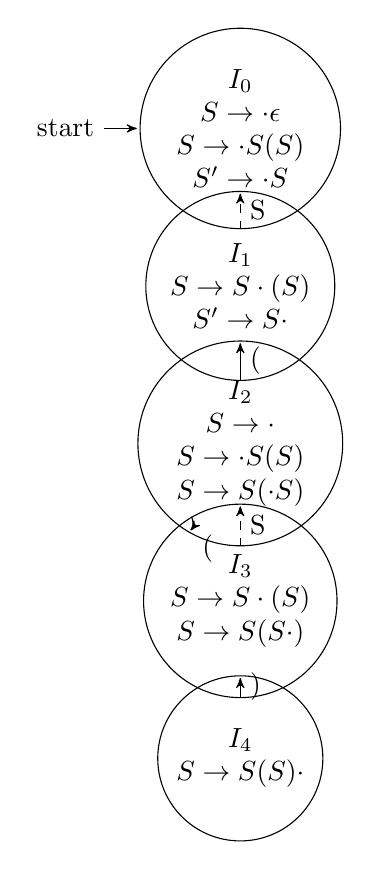
\begin{tikzpicture}[>=stealth',shorten >=1pt,auto,node distance=2cm,every text node part/.style={align=center}]
  \node[initial,state]  (i0)  {$I_0$ \\ $S \rightarrow  \cdot \epsilon$ \\ $S \rightarrow  \cdot S ( S )$ \\ $S' \rightarrow  \cdot S$};
  \node[state]  (i1)  [below of=i0]  {$I_{1}$ \\ $S \rightarrow  S \cdot ( S )$ \\ $S' \rightarrow  S \cdot $};
  \node[state]  (i2)  [below of=i1]  {$I_{2}$ \\ $S \rightarrow  \cdot $ \\ $S \rightarrow  \cdot S ( S )$ \\ $S \rightarrow  S ( \cdot S )$};
  \node[state]  (i3)  [below of=i2]  {$I_{3}$ \\ $S \rightarrow  S \cdot ( S )$ \\ $S \rightarrow  S ( S \cdot )$};
  \node[state]  (i4)  [below of=i3]  {$I_{4}$ \\ $S \rightarrow  S ( S ) \cdot $};
  \path[->,dashed] (i0) edge [right] node {S} (i1);
  \path[->] (i1) edge [right] node {(} (i2);
  \path[->,dashed] (i2) edge [right] node {S} (i3);
  \path[->] (i3) edge [bend left] node {(} (i2);
  \path[->] (i3) edge [right] node {)} (i4);
\end{tikzpicture}



% \begin{tikzpicture}[>=stealth',shorten >=1pt,auto,node distance=2cm,every text node part/.style={align=center}]
  \node[initial,state]  (i0)  {$I_0$};
  \node[state]  (i1)  [below of=i0]  {$I_{1}$};
  \node[state]  (i2)  [below of=i1]  {$I_{2}$};
  \node[state]  (i3)  [below of=i2]  {$I_{3}$};
  \node[state]  (i4)  [below of=i3]  {$I_{4}$};
  \node[state]  (i5)  [right of=i4]  {$I_{5}$};
  \node[state]  (i6)  [below of=i4]  {$I_{6}$};
  \node[state]  (i7)  [below of=i6]  {$I_{7}$};
  \path[->,dashed] (i0) edge [right] node {S} (i1);
  \path[->] (i1) edge [right] node {(} (i2);
  \path[->,dashed] (i2) edge [right] node {S} (i3);
  \path[->] (i3) edge [right] node {(} (i4);
  \path[->] (i3) edge [right] node {)} (i5);
  \path[->,dashed] (i4) edge [right] node {S} (i6);
  \path[->] (i6) edge [bend left] node {(} (i4);
  \path[->] (i6) edge [right] node {)} (i7);
\end{tikzpicture}



%\begin{tikzpicture}[shorten >=1pt,node distance=2cm,initial by arrow,initial where=above,initial text=,initial distance=1cm]
%  \node[initial,state,accepting] (S)      {$S$};
%  \node[state]         (q1) [right of=S,below of=S]  {$q_1$};
%  \node[state]         (q2) [right of=q1] {$q_2$};
%  
%  \path[->]          (S)  edge [loop above] node {a} (S);
%  \path[->, dashed]  (q1)  edge [loop above]  node {a} (q1);
%  \path[->, dashed]  (S)  edge              node {a} (q1);
%  \path[->, dotted]  (q1) edge [bend left]  node {a} (S);
%  \path[->>, dotted] (q1) edge             node {b} (q2);
%  \path              (q2) edge [loop above] node {b} (q2)
%             edge [bend left]  node {b} (q1);  
%\end{tikzpicture}

\section{Missing Features}

Some features are still waiting to be implemented or are improperly implented. This manual might even describe these features as implemented. A partial list of features or components in limbo:

% TODO: Add the list, will be a list of TODOs on the programming side.
\begin{itemize}
\item Either LR(0) or LALR(1) machines are incorrect.
\item The LR option does nothing.
\item Tikz is displaying terrible machines.
\item This manual is far from resembling a useful manual.
\item Tables for machines with memory, print an entry for each item in memory.
\end{itemize}

\section{Command Line Arguments}

The syntax for command line execution is


\indent \verb#java PTG Grammar [-Start symbol] [-End symbol] [-Empty symbol] #
\indent ~ ~ \verb#([-table [table_type] [out]] | [-machine [] [out]])+# 


\noindent or 


\indent \verb#java PTG grammar [-start symbol] [-end symbol] [-empty symbol] -all [out] # 


\noindent\verb#grammar# is the file that contains the grammar that will be parsed, it is a required argument and needs to be the first one supplied.

\noindent\verb#start# is an optional parameter which sets the start variable of the grammar to the supplied symbol. The default is the first variable listed in the grammar.

\noindent\verb#end# is an optional parameter which sets the end of input variable of the grammar to the supplied symbol. The default is \verb#$#.

\noindent\verb#empty# is an optional parameter which sets the empty string of the grammar to the supplied symbol. Default is \verb#<e>#.

\noindent\verb#symbol# a string that should avoid the symbol \verb|#| along with all whitespace.

\noindent\verb#table# should be replaced with one of

\indent\verb#first#
\indent\verb#follow#
\indent\verb#LL1#
\indent\verb#SLR1#
\indent\verb#LALR1#
\indent\verb#LR1#

\indent 

\section{Preparing the Input Grammar File}


\section{Implementing Generated Files}
\subsection{ \LaTeX{} Tables}
There are two simple ways to use generated \LaTeX{} tables, either by copy pasting or using the input command. PTG generates a tabular environment as opposed to an actual table environment, this is because a table (or other container, for example a figure) has commands that relate to placement of the environment in the document. The input command will allow the use of generated tex files directly. This allows a user to update a grammar file, run PTG for that grammar and then recompile the document. A table or figure environment can be used to contain the input command. Below is an example of how to insert a file named \tt{exampleTable.tex} into a figure:

\begin{figure}[h]
    \begin{minipage}{2in}
        \begin{verbatim}
            \begin{table}
            \centering
            %\input{exampleTable.tex}
            \caption{A caption for the table}
            \label{table:TableLabel}
            \end{table}
        \end{verbatim}
    \end{minipage}
\end{figure}

Both the caption and label commands are optional and the arguments supplied for them are nonsensical, \verb#\centering# is also optional.

\subsection{HTML Tables}
\subsection{Graphviz Statemachines}
Graphviz statemachine files have the extension .gz and should be rendered using Graphviz DOT. An example command to render exampleSM.gz as a png image file named exampleSM.png would be:


\indent\verb#.\dot -Tpng exampleSM.gz -o exampleSM.png#


\noindent Check the DOT documentation for more details. http://www.graphviz.org/pdf/dotguide.pdf

\section{I found a bug, what should I do?}

Sit tight, don't worry, we'll get through this. Send a few line describing what you were doing or intending to do, the command line inputs you used and the input grammar to [...]. //
If you can't wait, then feel free to modify the source code in hopes of fixing the bug.


\section{An Example}

\begingroup
\obeycr
%\input{example.gra}%
\endgroup%

\begin{table}[h]
    \begin{tabular}{l c r}
        \begin{minipage}{1in}
            %\input{exfirst.tex}
        \end{minipage}
        \qquad
        \begin{minipage}{1in}
            %\input{exfollow.tex}
        \end{minipage}
        \qquad
        \begin{minipage}{1in}
            %\input{exLL1.tex}
        \end{minipage}
    \end{tabular}
    \caption{\tt{FIRST}, \tt{FOLLOW} and \tt{LL(1)} parsing of the example}
    \label{table:ffex}
\end{table}

%\begin{figure}[h]
    %\includegraphics[scale=0.4]{exLR0.png}
    %\centering
    %\\
    %\input{exSLR1.tex}
    %\caption{\tt{LR(0)} and \tt{SLR(1)} of the example.}
    %\label{table:slrex}
%\end{figure}

%\begin{figure}[h]
    %\includegraphics[scale=0.4]{exLR1.png}
    %\centering
    %\\
    %\input{exLALR1.tex}
    %\caption{\tt{LALR(1)} of the example.}
    %\label{table:slrex}
%\end{figure}


\end{document}